\documentclass[table]{beamer}

% Layout: Copyright 2012 Dominik Wagenfuehr <dominik.wagenfuehr@deesaster.org>
% Dieses Dokument unterliegt der Creative-Commons-Lizenz
% "Namensnennung-Weitergabe unter gleichen Bedingungen 3.0 Deutschland"
% [http://creativecommons.org/licenses/by-sa/3.0/de/].

\usepackage[utf8]{inputenc}     % UTF8-Encoding
\usepackage[T1]{fontenc}        % T1-Schriftkodierung
\usepackage{lmodern}            % Ersetzung der CM-Schrift
\usepackage{ngerman}            % Deutsche Trennung
\usepackage{xifthen}            % if-Abfragen
\usepackage{textcomp}
    % Pakete einbinden
% Copyright 2012 Dominik Wagenfuehr <dominik.wagenfuehr@deesaster.org>
% Dieses Dokument unterliegt der Creative-Commons-Lizenz
% "Namensnennung-Weitergabe unter gleichen Bedingungen 3.0 Deutschland"
% [http://creativecommons.org/licenses/by-sa/3.0/de/].

%%%%%%%%%%%%%%%
% Coloring
%%%%%%%%%%%%%%%

\definecolor{basecolor}{RGB}{29,77,153}
\definecolor{secondcolor}{RGB}{246,249,252}
\definecolor{thirdcolor}{RGB}{255,255,255}

% infolines color
\setbeamercolor{palette primary}{fg=white,bg=basecolor}
\setbeamercolor{palette secondary}{fg=black,bg=secondcolor}
\setbeamercolor{palette tertiary}{fg=black,bg=thirdcolor}

% frame and title color
\setbeamercolor{frametitle}{fg=white,bg=basecolor}
\setbeamercolor{titlelike}{fg=white,bg=basecolor}
\setbeamerfont{frametitle}{series=\bfseries}

% TOC color
\setbeamercolor{section in toc}{fg=black}

% text color
\setbeamercolor{normal text}{fg=black,bg=white}

% item color
\setbeamercolor{item}{fg=basecolor}
\setbeamercolor{itemize item}{fg=basecolor}

%%%%%%%%%%%%%%%
% Theme
%%%%%%%%%%%%%%%

% Theme-Auswahl
\useinnertheme{rectangles}
\useoutertheme{infolines}
\usecolortheme{default}
\usefonttheme{default}

%%%%%%%%%%%%%%%
% Template
%%%%%%%%%%%%%%%

% Keine Navigationssymbole
\setbeamertemplate{navigation symbols}{}

% opaque preview of further text on sheet
\setbeamercovered{invisible}

% Headline
\setbeamertemplate{headline}
{%
    %empty
}

% Footline
\setbeamertemplate{footline}
{%
    \begin{beamercolorbox}[dp=3px,ht=6px,wd=\paperwidth,left]{palette secondary}%
        \setlength{\fboxsep}{0pt}%
        \parbox{2.1cm}{\centering{}\insertdate{}}%
        \ifthenelse{\boolean{showcclicense}}{%
            \parbox{6.7cm}{\centering{}\inserttitle{} – \insertsubtitle{}}%
            \parbox{2.5cm}{\centering{}Seite \insertframenumber{} von \inserttotalframenumber{}}%
            \parbox{1.5cm}{\centering{}\href{http://creativecommons.org/licenses/by-sa/3.0/deed.de}{
\includegraphics[height=6px]{images/cc-by-sa.pdf}}}%
        }{%
            \parbox{8.2cm}{\centering{}\inserttitle{} – \insertsubtitle{}}%
            \parbox{2.5cm}{\centering{}Seite \insertframenumber{} von \inserttotalframenumber{}}%
        }
    \end{beamercolorbox}%
    \vspace*{4px}%
}

% Frametitle
\setbeamertemplate{frametitle}
{%
    \ifthenelse{\boolean{showframesubtitle}}{%
        \vspace*{-1px}\hspace*{-11px}%
        \begin{beamercolorbox}[dp=4px,ht=34px,wd=39px,left]{palette primary}%
            \hspace*{3px}%
            
\includegraphics[width=32px]{images/logo_weiss_klein.pdf}%
        \end{beamercolorbox}
        
        \vspace*{-39px}\hspace*{27px}%
        \begin{beamercolorbox}[dp=8px,ht=30px,wd=325px,left]{palette primary}%
            \hspace*{5px}%
            \insertframetitle{}\\[-0.4em]%
            \hspace*{5px}%
            {\footnotesize \insertframesubtitle{}}%
        \end{beamercolorbox}%
    }{%
        \vspace*{-1px}\hspace*{-11px}%
        \begin{beamercolorbox}[dp=4px,ht=28px,wd=32px,left]{palette primary}%
            \hspace*{2px}%
            
\includegraphics[width=26px]{images/logo_weiss_klein.pdf}%
        \end{beamercolorbox}
        
        \vspace*{-33px}\hspace*{20px}%
        \begin{beamercolorbox}[dp=10px,ht=22px,wd=332px,left]{palette primary}%
            \hspace*{5px}%
            \insertframetitle{}%
        \end{beamercolorbox}%
    }%
}

% Titelseite
\setbeamertemplate{title page}
{%
    \begin{beamercolorbox}[sep=10px,wd=\linewidth,right]{transparent}%
        
\includegraphics[width=120px]{images/logo_blau_gross.pdf}%
    \end{beamercolorbox}%

    \vspace*{4em}%
    \begin{beamercolorbox}[sep=10px,wd=\linewidth,center]{palette primary}%
        {\LARGE\inserttitle{}}\\[0.5em]
        {\large\insertsubtitle{}}
    \end{beamercolorbox}%

    \vspace*{3em}%
    \begin{beamercolorbox}[wd=\linewidth,center]{transparent}%
        \insertauthor{}\\[0.2em]%
        \insertinstitute{}~\\[0.5em]%
        \insertdate{}%
    \end{beamercolorbox}%
}
    % Layout
% Copyright 2012 Dominik Wagenfuehr <dominik.wagenfuehr@deesaster.org>
% Dieses Dokument unterliegt der Creative-Commons-Lizenz
% "Namensnennung-Weitergabe unter gleichen Bedingungen 3.0 Deutschland"
% [http://creativecommons.org/licenses/by-sa/3.0/de/].

% CC-Lizenz ein- oder ausblenden
\newboolean{showcclicense}
\setboolean{showcclicense}{false}
\newcommand*{\ShowCCLicense}[1][true]{%
    \setboolean{showcclicense}{#1}%
}

% Frame-Subtitle ein- oder ausblenden
\newboolean{showframesubtitle}
\setboolean{showframesubtitle}{false}
\newcommand*{\ShowFrameSubtitles}[1][true]{%
    \setboolean{showframesubtitle}{#1}%
}


% Box-Definitionen
\definecolor{dunkelgrau}{gray}{0.35}
\definecolor{hellgrau}{gray}{0.93}
\definecolor{hellgelb}{rgb}{1.0,1.0,0.9}

\newcommand{\ListingBox}[1]
{%
    \begin{small}
        \begin{semiverbatim}
            \fcolorbox{dunkelgrau}{hellgelb}{%
                \begin{minipage}{0.965\linewidth}
                    #1
                \end{minipage}
            }
        \end{semiverbatim}
    \end{small}
}

\newcommand{\CommandBox}[1]
{%
    \begin{small}
        \begin{semiverbatim}
        \fcolorbox{dunkelgrau}{hellgrau}{%
            \begin{minipage}{0.965\linewidth}
                #1
            \end{minipage}
        }
        \end{semiverbatim}
    \end{small}
}
   % Befehle einbinden

\title{Homeserver}
\subtitle{Selber bauen}
\author{Stefan J. Betz}
\institute{Backspace e.V.}
\date{24. Oktober 2015}
\subject{Wir bauen einen Homeserver}
\keywords{Linux, Homeserver, Sicherheit, Software, Hardware, Backup}

% Dies hier auskommentieren, wenn man den CC-Verweis im Dokument
% nicht haben will.
\ShowCCLicense{}

% Dies auskommentieren, wenn auf den einzelnen Folien keine
% Frame-Subtitle gezeigt werden sollen.
\ShowFrameSubtitles{}

\begin{document}

\begin{frame}[t,plain]
\titlepage
\end{frame}

\begin{frame}
\frametitle{Inhalt}
\tableofcontents[hideallsubsections]
\end{frame}


\section{about:me}

\begin{frame}{about:me}
\framesubtitle{Ausweis bitte.}
\begin{itemize}
\item \textasciitilde{}1984 geboren
\pause
\item \textasciitilde{}2000 mit dem Thema Homeserver angefangen
\pause
\item \textasciitilde{}2010 Serverteam bei ubuntuusers.de…
\pause
\item …was auch Ubuntu Iran, Ubuntu Deutschland e.V., Teile von Ubuntu Berlin, etc… bedeutet
\end{itemize}
\end{frame}

\section{Hardware}

\begin{frame}{RAM}
\framesubtitle{RAM ist nur durch noch mehr RAM zu ersetzen!}
\begin{itemize}
\item 1GB für Fileserver…
\pause
\item … vergesst ZFS und btrfs
\pause
\item 2GB für Webserver…
\pause
\item …vergesst Java
\pause
\item 4GB+ für File-, Webserver und kleinen VM Host
\end{itemize}
\end{frame}

\begin{frame}{CPU}
\framesubtitle{80386 könnte ggf. eng werden.}
\begin{itemize}
\item Intel vs. AMD = Religion.
\pause
\item AES-NI = Verschlüsselung
\pause
\item 64-Bit, weil RAM
\end{itemize}
\end{frame}

\begin{frame}{Intel Core i3 vs. Atom}
\framesubtitle{Verschlüsselung}
\begin{figure}
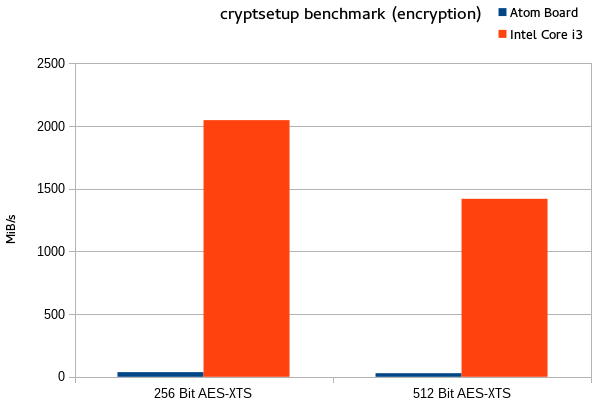
\includegraphics[width=0.8\textwidth]{images/cryptsetup-benchmark.png}
\caption{cryptsetup benchmark}
\end{figure}
\end{frame}

\begin{frame}{Intel Core i3 vs. Atom}
\framesubtitle{Kompression}
\begin{figure}
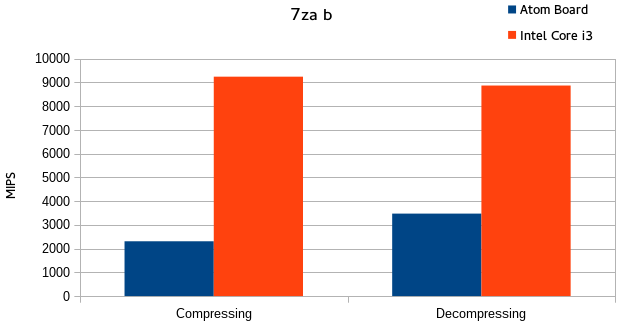
\includegraphics[width=0.8\textwidth]{images/7zab-benchmark.png}
\caption{7za b}
\end{figure}
\end{frame}

\begin{frame}{Storage}
\framesubtitle{Catcontent braucht Platz}
\begin{itemize}
\item SATA ist alternativlos
\pause
\item SSDs zu teuer
\pause
\item Backup > RAID
\pause
\item Wechselrahmen
\pause
\item RAID Levels (sinnvoll): 1, 5, 6
\pause
\item LVM
\end{itemize}
\end{frame}

\begin{frame}{Diverses}
\framesubtitle{Kleinigkeiten}
\begin{itemize}
\item Desktop Boards ohne Extras taugen
\pause
\item Stromverbrauch wird oft überschätzt
\pause
\item Netzteil nicht zu groß kaufen
\end{itemize}
\end{frame}

\section{Software}

\begin{frame}{Software}
\framesubtitle{Distrowar - Debian}
\begin{itemize}
\item LTS Status noch Neuland
\pause
\item Upgrades zeitlich unbestimmt, ca. ~2 Jahre
\end{itemize}
\end{frame}

\begin{frame}{Software}
\framesubtitle{Distrowar - Ubuntu}
\begin{itemize}
\item LTS Status für 5 Jahre…
\pause
\item …gilt nur für \tt{main} Repository
\end{itemize}
\end{frame}

\begin{frame}{Software}
\framesubtitle{Distrowar - CentOS}
\begin{itemize}
\item Updates für 10 Jahre
\pause
\item SELinux
\pause
\item Alte Software
\end{itemize}
\end{frame}

\begin{frame}{Software}
\framesubtitle{Distrowar - Arch}
\begin{itemize}
\item Rolling Release
\pause
\item Software (inkl. Bugs) stets aktuell
\end{itemize}
\end{frame}

\section{Backups}

\begin{frame}{Backup: Grundlagen}
\framesubtitle{Allegemeine Sicherheitshinweise}
\begin{enumerate}
\item Online (Platte, NAS, Cloud, …) zählt nur bedingt als Backup
\pause
\item 2 Kopien der Daten, an unterschiedlichen Orten
\pause
\item Daten die nicht gesichert sind, sind auch nicht wichtig
\pause
\item Backups automatisch, Menschen machen keine Backups, Maschinene schon
\pause
\item Backup (Medium, Dateisystem, Daten) regelmäßig prüfen
\end{enumerate}
\pause
\textbf{Worst Case}: Hausbrand, Blitzeinschlag, Diebstahl, Dummheit
\end{frame}

\begin{frame}{Backup: Wichtiges/Unwichtiges}
\framesubtitle{Ersetzbares kann ersetzt werden}
\pause
\textbf{Wichtig}
\begin{itemize}
\item Familienfotos => Unersetzbare Erinnerungen
\pause
\item Mails => Ermöglichen Zugang zu Online Diensten
\pause
\item GPG / SSH Keys => Ermöglichen Lesen von Mails oder Zugang zu Servern (!)
\pause
\item Rechnungen, Mahnungen, bzw. Lebensrelevanter Schriftverkehr
\end{itemize}
\pause
\textbf{Unwichtig}
\begin{itemize}
\item Betriebssystem
\pause
\item ISO Images
\pause
\item Catcontent, P0rn, Warez
\end{itemize}
\end{frame}

\section{Aufwand}

\begin{frame}{Aufwand}
\framesubtitle{Zeit ist Geld}
Faustformel:
\begin{itemize}
\item Pro Dienst bzw. Anwendung ca. 1 Stunde pro Monat
\pause
\item Pro Maschine (auch VMs, Container, …) ca. 1 Stunde pro Monat
\end{itemize}
\end{frame}

\begin{frame}{Aufwand}
\framesubtitle{Woher kommt Aufwand?}
\begin{itemize}
\item Updates
\pause
\item Backups
\pause
\item Webanwendungen (und deren Abhängigkeiten)
\pause
\item Ausfälle (Shit happens)
\end{itemize}
\end{frame}

\begin{frame}{Aufwand}
\framesubtitle{TDP als Energie}
TDP != Stromverbrauch, sondern:\\
\pause
\begin{quote}
Mit Thermal Design Power wird in der Elektronikindustrie ein maximaler Wert für die thermische Verlustleistung … elektronischer Bauteile bezeichnet, auf deren Grundlage die Kühlung sowie die Stromzufuhr ausgelegt werden.
\end{quote}
\begin{small}
Quelle: Wikipedia
\end{small}
\end{frame}

\begin{frame}{Aufwand}
\framesubtitle{Was kostet Energie}
Energiekosten: 29 Cent/KWh, als Dauerlast:\\
\pause
\begin{tabular}{|l|r|r|}
\hline
\textbf{Leistung} & \textbf{Jahr} & \textbf{Monat} \\
\hline
50 Watt & 127€ &  10€ \\
\hline
35 Watt & 89€ & 7.50€ \\
\hline
15 Watt & 38€ & 3.20€ \\
\hline
\end{tabular}
\pause
\begin{itemize}
\item Intel Core i3 4130T, Gigabyte H87-HD3, 400 Watt 80+ NT => \textasciitilde{}25 Watt Idle
\pause
\item GA-D525TUD (Atom CPU!) => \textasciitilde{}15-20 Watt Idle
\pause
\item Speedport W723V Typ B 7.0-8.5 Watt (je nach DECT/WLAN)
\end{itemize}
\end{frame}

\begin{frame}{Aufwand}
\framesubtitle{Energieverbrauch von Festplatten}
\begin{tabular}{|l|r|r|r|l|r|}
\hline
\textbf{Platte}   & \textbf{Standby} & \textbf{Idle} & \textbf{Work} & \textbf{Garantie} & \textbf{Euro (1TB)} \\
\hline
WD Green &     0.4 &  2.5 &  3.3 & 2 Jahre  &        47€ \\
\hline
WD Red   &     0.4 &  2.3 &  3.3 & 3 Jahre  &        60€ \\
\hline
WD RE4   &       - &  5.9 &  8.6 & 5 Jahre  &        90€ \\
\hline
WD VR    &     1.1 &  4.2 &  5.8 & 5 Jahre  &       300€ \\
\hline
WD Black &     0.8 &  6.1 &  6.8 & 5 Jahre  &        73€ \\
\hline
\end{tabular}
\end{frame}


\begin{frame}[t]
    \frametitle{~}

    \begin{center}
        \ifthenelse{\boolean{showcclicense}}{%
            \vspace*{3em}%
            Vielen Dank für die Aufmerksamkeit!\\[2em]
            \begin{scriptsize}
                Die Folien unterliegen der
                \href{http://creativecommons.org/licenses/by-sa/3.0/deed.de}{CreativeCommons \\
                "`Namensnennung-Weitergabe unter gleichen Bedingungen 3.0 Unported"'.\\[1em]
                
\includegraphics[scale=0.5]{images/cc-by-sa-gross.pdf}}\\[2em]
                
                2014 \insertauthor{}
            \end{scriptsize}
        }{%
            \vspace*{5em}%
            Vielen Dank für die Aufmerksamkeit!\\[8em]
        }
    \end{center}

    \begin{beamercolorbox}[sep=10px,wd=\linewidth,right]{transparent}%
        
\includegraphics[width=120px]{images/logo_blau_gross.pdf}%
    \end{beamercolorbox}%

\end{frame}    


\end{document}
